\documentclass{mytex}
\usepackage{xcolor}
\usepackage{fontawesome5}
\usepackage{babel}
\usepackage{tcolorbox}
\usepackage{uml} % Ce package permet des diagrammes UML simples
\tcbuselibrary{skins, listings}
\newtcblisting{codebox}{   
	enhanced, 
	colback=black!3!white, 
	toprule=1pt, 
	bottomrule=1pt, 
	leftrule=0pt, 
	rightrule=0pt, 
	arc=0mm, 
	attach boxed title to top left={yshift=-9pt, xshift=4pt},
	title = Java,
	coltitle=black, 
	boxed title style={colback=white},
	listing only,
	fontupper=\footnotesize, % réduction de la taille du code
	listing options={
		language=java,
		breaklines,
		keywordstyle=\color{red!60!black},
		keywordstyle={[2]\color{orange}},
		commentstyle=\color{gray}\itshape,
		stringstyle=\color{blue},
		showstringspaces=false,
		numbers=left,
		numberstyle=\tiny,
		stepnumber=1,
		numbersep=10pt % réduit l'espace entre le code et les numéros
	},
}

% pour les accents
\lstset{
	literate=
		{é}{{\'e}}1
		{è}{{\`{e}}}1
		{ê}{{\^{e}}}1
		{ë}{{\¨{e}}}1
		{É}{{\'{E}}}1
		{Ê}{{\^{E}}}1
		{û}{{\^{u}}}1
		{ù}{{\`{u}}}1
		{â}{{\^{a}}}1
		{à}{{\`{a}}}1
		{Â}{{\^{A}}}1
		{ç}{{\c{c}}}1
		{Ç}{{\c{C}}}1
		{ô}{{\^{o}}}1
		{Ô}{{\^{O}}}1
		{î}{{\^{i}}}1
		{Î}{{\^{I}}}1,
}

\title{Rapport ECL - Template} %Titre du fichier

\begin{document}



%----------- Informations du rapport ---------

\titre{Conception \& Développement} %Titre du fichier .pdf
\UE{SAÉ S2.01-02} %Nom de la UE
\sujet{Programmation orientée objet} %Nom du sujet

\enseignant{Antoine \textsc{Nongaillard} \\ Fabien \textsc{Delecroix}} %Nom de l'enseignant

\eleves{Baptiste \textsc{Lavogiez} \\
		Mark \textsc{Zavadskiyi} \\ 
		Angèl \textsc{Zheng}} %Nom des élèves

%----------- Initialisation -------------------
        
\fairemarges %Afficher les marges
\fairepagedegarde %Créer la page de garde
\tabledematieres %Créer la table de matières

%------------ Corps du rapport ----------------


Ce rapport présentera la partie \textbf{Conception \& Développement} de la SAÉ S2.01-02. Elle traitera d'une solution à la situation d'échange scolaire entre deux personnes régie par des critères et exigences formulées ou non.

\section{Rendu 1}

Ce premier rendu traitera de la conception des classes des bases, des contraintes et des classes de tests.

\subsection{Réflexion}

Cette semaine, nous avons à poser les bases de notre projet.
Nous réflechissons d'abord aux structures les plus adaptées pour le besoin, qui est ici d'échanger des élèves entre eux sur la base de critères.

Nous avons besoin d'une Personne, de Critères stockés avec leur types, et d'un Echange entre deux Personnes.
Cela se matérialise avec un UML.

\subsection{UML}

\insererfigure{img/uml_v1.png}{12cm}{Relations UML}{Label de la figure}

\subsection{Remarques}

Nous avons décidé d'une représentation minimaliste mais avec tous les éléments nécessaires.
Le code est facilement compréhensible avec des noms explicites.

\tsec{Des critères...}

Criteria est une énumération simple de critères associés à un type représenté sous forme de caractère.

Cette énumération est utilisée dans criteriaValues, la Map de la classe Person. Elle y sera associée à une valeur représentée en chaîne de caractères pour simplifier la modélisation. Dans Person, les méthodes adéquates permettent de manipuler ces critères (ajout, obtention, conversion en texte...).

Dans cette Map, chaque clef correspond à un critère et sa valeur représente son résultat. De plus, les méthodes de la classe Person permettent d'accéder aux critères d'une personne.

\tsec{Person ou Student ?}

Ici, le fait que les personnes soient des étudiants n'est pas important.
Choisir le modèle d'un étudiant reviendrait à devoir encapsuler une personne dans la classe, soit une classe de plus.

\tsec{Le double rôle}

Une personne peut aussi bien être un hote qu'un guest.
Pour cela, Exchange encapsule les deux afin d'avoir une combinaison claire et simple à manipuler.

\tsec{Critiques}

La classe Exchange aurait pu, de façon plus ou moins simple, se raccourcir en étant définie dans Person.
Le problème étant que de cette façon, le rôle de Host et de Guest devrait être défini autrement. Nous préférons Exchange pour fonctionner de manière plus simple afin de manipuler clairement les rôles.

\subsection{Implémentation}

L'implémentation se fait de manière naturelle après avoir tout défini de façon claire.
Des tests élargis sont disponibles dans le dossier sous-jaçent et permettent de voir comment le modèle réagit à toutes les situations.

\tsec{Aperçu de Exchange}

\begin{codebox}
package v1;

public class Exchange {
    private Person host;
    private Person guest;

    public Exchange(Person host, Person guest) {
        this.host = host;
        this.guest = guest;
    }

    public Person getHost() {
        return this.host;
    }

    public Person getGuest() {
        return this.guest;
    }
\end{codebox}

\tsec{Aperçu de ExchangeTest}

\begin{codebox}
package v1 ; 

public class ExchangeTest {

    private Person alice;
    private Person bob;
    private Exchange exchange;

    @BeforeEach
    public void initTest() {
        alice = new Person("Astana", "Nur-sultan");
        bob = new Person("Bob", "Marley");
        exchange = new Exchange(alice, bob);
    }

    @Test
    public void testIncompatibleDueToAnimalAllergy() {
        alice.addCriteriaValue(Criteria.HOST_HAS_ANIMAL, "true");
        bob.addCriteriaValue(Criteria.GUEST_ANIMAL_ALLERGY, "true");

        assertFalse(exchange.isCompatible());
    }

    @Test
    public void testIncompatibleDueToGenderPreference() {
        alice.addCriteriaValue(Criteria.HOST_HAS_ANIMAL, "false");
        bob.addCriteriaValue(Criteria.GUEST_ANIMAL_ALLERGY, "false");
        alice.addCriteriaValue(Criteria.PREFERENCE_GENDER, "Female");
        bob.addCriteriaValue(Criteria.GENDER, "Male");

        assertFalse(exchange.isCompatible());
    }
\end{codebox}

\section{Rendu 2}

\subsection{Attentes}

Cette semaine, nous traiterons de : 

\begin{itemize}
	\item Gestion de la validité des critères par un mécanisme d’exception
	\item Développement des règles spécifiques de compatibilité pour certains pays
\end{itemize}

La règle spécifique de compatibilité étant, pour le moment, celle énonçant qu'un échange comprenant une personen française devait avoir au moins un hobby en commun sans quoi le risque de cassure serait trop important.

La validité des critères portera sur :

\begin{itemize}
	\item La bonne entrée d'un type (car jusqu'ici ils sont tous en String) ; exemple : HOST\_HAS\_ANIMAL doit être à true ou false.
	\item La cohérence des valeurs entrées. Par exemple une Person ne peut pas être allergique aux animaux et en avoir un.
\end{itemize}

\subsection{Réflexion}

Nous avons réfléchi à comment implémenter les critères spécifiques aux pays.

Nous avons pensé à :

\begin{itemize}
	\item Une énumération \texttt{SpecificCountryRule}
	\item Une ArrayList de "rules" au sein de \texttt{Person}
\end{itemize}

Au final, nous avons opté pour une définition dans \texttt{Person} au sein de la liste de critères.

La validité des critères, elle, a été validée en divisant la vérification en deux temps : d'abord le bon respect du type prévu (pas de \texttt{yes} dans un boolean), pour ensuite vérifier la bonne valeur (pas de \texttt{toto} dans la date de naissance).

\subsection{UML}

L'UML est, par conséquent, mis à jour et amélioré dans ses détails.

\insererfigure{img/uml_v2.png}{11cm}{Relations UML}{fig::v2::uml}

\subsection{Modifications de \texttt{Person}}

Pour ce faire, nous avons procédé à l'implémentation d'une méthode \texttt{meetingSpecificCountryRules} dans la classe \texttt{Person}.

Elle est appelée dans le constructeur désormais surchargé et à l'ajout d'un nouveau critère. En somme, elle est appelée à chaque possible changement de critère pour adapter la bonne logique.

\begin{codebox}
    // Cette méthode change les critères en fonction du pays
	// Elle doit être appelée à chaque fois qu'on change un critère (constructeur, ajout)
public void meetingSpecificCountryRules() {
	try {
		String country = this.getCriteriaValue(Criteria.COUNTRY_OF_ORIGIN).toUpperCase();
		if (country.equals("FRANCE")) {
			this.addCriteriaValue(Criteria.NEED_ONE_HOBBY, "true");
		}
	} catch (NullPointerException e) {
		// Si le pays n'est pas défini, on ne fait rien, ce n'est pas vraiment une erreur
	}
}
\end{codebox}

Dans la même idée et dans la même classe, une méthode \texttt{isThereIncoherence} a été ajoutée. Elle veille à faire respecter les contradictions de données ; ici, il est sujet d'une personne allergique aux animaux mais en ayant un aussi en même temps.

\begin{codebox}
public boolean isThereIncoherence() {
	// On vérifie si la personne a un animal et est allergique
	String hostHasAnimal = this.getCriteriaValue(Criteria.HOST_HAS_ANIMAL);
	String guestAllergy = this.getCriteriaValue(Criteria.GUEST_ANIMAL_ALLERGY);
	
	if ("true".equals(guestAllergy) && "true".equals(hostHasAnimal)) {
		return true;
	}
	return false;
}
\end{codebox}

De plus, une \texttt{ArrayList} de \texttt{hobbies} a été ajoutée, en accord avec les critères relatifs à un nombre de hobbies en commun minimal.

\subsection{Modifications de \texttt{Criteria}}

Un critère a été ajouté : \texttt{NEED\_ONE\_HOBBY}, caractérisant le besoin dans un \texttt{Exchange} d'avoir au moins un hobby en commun en cas de règles spécifiques. Ce critère est un booléen ('B').

La vérification des critères se décompose en deux parties : type, puis valeur.

\tsec{La méthode \texttt{static isCriteriaTypeValid}}

\begin{codebox}
public static boolean isCriteriaTypeValid(Criteria criteria, String value) {
	char type = criteria.getType();
	switch(type) {
		case 'B':
		value = value.toLowerCase(); // on met tout en minuscule
		// On vérifie si la valeur est "true" ou "false"
		return value.equals("true") || value.equals("false");
		case 'T':
		return (value.length()>0); // TODO: Add validation for text criteria
		case 'N':
		try {
			Integer.parseInt(value);
			return true;
		} catch (NumberFormatException e) {
			System.out.println("Invalid number format: " + value);
			System.out.println("Exception: " + e.getMessage());
			return false;
		}
		case 'D':
	}
	return false;
}
\end{codebox}

Cette méthode sera appelée, en complément de la suivante, à chaque nouvel ajout de critère. Si les méthodes ne sont pas satisfaites, l'ajout échoue et une exception est lancée pour signaler que le critère n'est pas valide.

\tsec{La méthode \texttt{static isCriteriaValueValid}}

\begin{codebox}
public static boolean isCriteriaValueValid(Criteria criteria, String value) {
	value = value.toLowerCase(); // on met tout en minuscule
	// Mode en if car pas toutes les valeurs sont concernées
	if(criteria==Criteria.PREFERENCE_GENDER || criteria==Criteria.GENDER) return value.equals("male") || value.equals("female") || value.equals("other");
	if(criteria==Criteria.DATE_OF_BIRTH) {
		try {   //Cette partie gestion d'excception est plutôt à mettre lors de l'entrée des données.
			return LocalDate.now().minusYears(18).isAfter((LocalDate.parse(value)));
		} catch (DateTimeParseException e) {
			System.out.println("Format invalide, utilisez le format suivant : yyyy-MM-dd."); 
			return false;
		}
	}   
	return true ;
}
\end{codebox}

\tsec{La méthode \texttt{static areCriteriasValid}}

\begin{codebox}
    // Vérifie l'ensemble des critères et leur validité. Si un n'est pas valide, on renvoie false.
public static boolean areCriteriasValid(Map<Criteria, String> criterias) {
	for (Map.Entry<Criteria, String> entry : criterias.entrySet()) {
		Criteria criteria = entry.getKey();
		String value = entry.getValue();
		try {
			if (!isCriteriaTypeValid(criteria, value)) {
				System.out.println("Invalid type for criteria " + criteria + ": " + value);
				return false;
			}
		} catch (Exception e) {
			System.out.println("Exception during type validation for " + criteria + ": " + e.getMessage());
			return false;
		}
		try {
			if (!isCriteriaValueValid(criteria, value)) {
				System.out.println("Invalid value for criteria " + criteria + ": " + value);
				return false;
			}
		} catch (Exception e) {
			System.out.println("Exception during value validation for " + criteria + ": " + e.getMessage());
			return false;
		}
	}
	return true;
}
\end{codebox}

Cette méthode est appelée dans le constructeur prenant en entrée une la \texttt{Map} des critères de la \texttt{Person}.

Les critères fournis sont valides et ont été vérifiés lors de l'instanciation de la classe Person.
	
\subsection{Modifications de \texttt{Exchange}}

\tsec{La méthode \texttt{countCommonHobbies}}

\begin{codebox}
//Donne le nombre de centre d'interêt en commun
//Dans le cadre du critère "NEED_ONE_HOBBY"
public int countCommonHobbies(){
	ArrayList<String> hostHobbies = this.host.getHobbies();
	ArrayList<String> guestHobbies = this.guest.getHobbies();
	int commonHobbies = 0;
	for (String hobby : hostHobbies) {
		if (guestHobbies.contains(hobby)) {
			commonHobbies++;
		}
	}
	return commonHobbies;
}
\end{codebox}

Cette méthode est utilisée afin de satisfaire ou non le critère \texttt{NEED\_ONE\_HOBBY}.

\tsec{Adaptation de \texttt{isCompatible}}

\begin{codebox}
	public boolean isCompatible() {
		...
		...
		String hostHobbies = this.host.getCriteriaValue(Criteria.NEED_ONE_HOBBY);
		String guestHobbies = this.guest.getCriteriaValue(Criteria.NEED_ONE_HOBBY);
		if(!this.host.getHobbies().isEmpty() && !this.guest.getHobbies().isEmpty() && (hostHobbies.equals("true") || guestHobbies.equals("true")) && countCommonHobbies() < 1){
			return false;
		}
		return true;
	}
\end{codebox}

Nous avons implémenté la gestion de la règle spécifiant que les paires avec une \texttt{Person} avec pour pays \texttt{France}, il faut au moins un hobby en commun. Pour ce faire, nous appelons la fonction précédemment définie \texttt{countCommonHobbies}

\subsection{Classes de Test}

Les classes \texttt{ExchangeTest} ainsi que \texttt{PersonTest} ont été mises à jour conformément aux ajouts.

De plus, la classe \texttt{CriteriaTest} fait son apparition.

\begin{codebox}
public class CriteriaTest {
	
	private Person alice;
	
	@BeforeEach
	void setUp() {
		alice = new Person("Alice", "Smith");
		alice.addCriteriaValue(Criteria.HOST_HAS_ANIMAL, "true");
		alice.addCriteriaValue(Criteria.PREFERENCE_GENDER, "Female");
	}
	
	@Test
	void testCriteriaTypeValid() {
		assertTrue(Criteria.isCriteriaTypeValid(Criteria.HOST_HAS_ANIMAL, "true"));
		assertFalse(Criteria.isCriteriaTypeValid(Criteria.HOST_HAS_ANIMAL, "yes"));
		assertTrue(Criteria.isCriteriaTypeValid(Criteria.PREFERENCE_GENDER, "male"));
		assertFalse(Criteria.isCriteriaTypeValid(Criteria.COUNTRY_OF_ORIGIN, ""));
	}
	
	@Test
	void testCriteriaValueValid() {
		assertTrue(Criteria.isCriteriaValueValid(Criteria.PREFERENCE_GENDER, "male"));
		assertFalse(Criteria.isCriteriaValueValid(Criteria.PREFERENCE_GENDER, "femme"));
		assertTrue(Criteria.isCriteriaValueValid(Criteria.DATE_OF_BIRTH, "2000-01-01"));
		assertFalse(Criteria.isCriteriaValueValid(Criteria.DATE_OF_BIRTH, "2020-01-01"));
		assertFalse(Criteria.isCriteriaValueValid(Criteria.DATE_OF_BIRTH, "je suis le 8 mai 1212 et je suis mal écrit"));
	}
}	
\end{codebox}

\section{Rendu 3}

\subsection{Attentes}

Ces deux semaines de réalisation seront les plus denses !

Au programme, nous avons :

\begin{itemize}
	\item Import par fichier de format csv, répondant à la structure donnée
	\item Export d’un résultat sous format csv
	\item Gestion de l’historique par sérialisation binaire
	\item Implémentation d’un jeu de données montant le bon fonctionnement du nouveau système d’affectation
\end{itemize}

Bonne nouvelle, \textbf{nous avons tout réalisé !}

D'autres changements mineurs : 
Les commentaires dans le code ont été \textbf{réécrits en anglais} afin que le projet, une fois visible sur notre portfolio, ait une plus grande portée.

Avant d'aller tête la première dans notre IDE favori, il est important de réfléchir à comment nous allons implémenter ces attentes. 

\subsection{Réflexion}

A l'issue de ce rendu, la partie POO de ce projet sera quasiment terminée. Ainsi, il est important de considérer les attentes de la partie IHM et de produire du code réutilisable dans JavaFX.

Traitons les attentes une par une et trouvons-y une procédure de traitement : 

\tsec{Import de CSV}

Nous devons ici lire un CSV contenant les personnes sujettes à de futurs échanges !

La forme du CSV est donnée dans le sujet à la fin.
Une petite retouche mineure a été de renommer les critères de façon à ce qu'ils aient le même nom que celui de la forme. Cela ne change rien au code, mais il est largement préférable que les deux aient le même nom.

Ensuite, une fonction \textbf{readCSV()} a été imaginée, avec un mécanisme de \textit{try with resources} pour s'habituer à une lecture propre.

L'idée sera ensuite de recréer les attributs de la personne un par un pour ensuite appeler le constructeur de Person avec ces attributs.

\tsec{Export d'un résultat en CSV}

L'objectif ici est d'exporter les meilleurs échanges.
Nous pensons y mettre : Le pays hôte, le pays visiteur, les dates et quelques informations sur les personnes, pour finir par le score.

\tsec{Gestion de l'historique par sérialisation binaire}

Après avoir été introduit à la sérialisation en cours, nous devrions être en mesure de pouvoir sérialiser un objet List<Exchange> de tous les échanges passés (soit tous ceux considérés comme les meilleurs avec une date de fin antérieure à aujourd'hui). Le reconstruire permettra de l'appliquer à un objet List<Exchange> history de type static accessible partout. Dans la classe Exchange, nous comparerons l'effectif de l'échange actuel (this) à ceux passés.

\tsec{Implémentation d'un jeu de données}

Tout au long du développement, nous testerons des jeux de données d'une structure identique à celle donnée. Ils seront décrits et appliqués lors de tests !

\subsection{UML}

Les classes, qu'elles soient nouvelles ou modifiées, sont présentées ci-dessous.

\insererfigure{img/version3/uml.png}{22cm}{Relations UML}{fig::v3::uml}

Attaquons-nous maintenant à la description de tous ces changements.

\obs{Des commentaires ont été retirés du code affiché en extraits afin de le raccourcir. Les fichiers de code contiendront alors plus d'informations qu'ici et sont disponibles pour éclaircir tout manque de clarté.}

\obs{L'ordre de présentation est également important et nous essayons de présenter les éléments avant qu'ils soient utilisés ailleurs.}

\subsection{Nouveau dossier : res}

Ce dossier, nommé par convention, contiendra nos fichiers CSV, contenant les informations nécessaires à la construction de futurs objets Person.

\insererfigure{img/version3/arbo.png}{3cm}{Arborescence des éléments}{fig::v3::arbo}

\begin{itemize}
	\item data, contenant les données prises en entrée
	\item results, contenant les données en sortie (exportation CSV, sérialisation)
\end{itemize}

Les fichiers CSV contiennent tous le même en-tête, tandis que le fichier sérialisé ne contient que du binaire, ne nécessitant donc aucune extension.

\insererfigure{img/version3/apercufichier.png}{8cm}{Aperçu du contenu d'un fichier data}{fig::v3::apercufichier}

\subsection{Nouvelle classe : CountryVisit}

Il est temps que les visites entre pays aient maintenant leur propre classe !
Cette classe a pour objectif d'inclure un pays hôte et un pays visiteur, avec une liste de personnes des pays mentionnés. Ensuite, il conviendra de déterminer les meilleurs échanges en appelant la gestion du score d'affinité dans la classe Exchange.

\tsec{Les attributs}

\begin{codebox}
private String guestCountry;
private String hostCountry;

private List<Person> guestPersons = new ArrayList<>();
private List<Person> hostPersons = new ArrayList<>();

// Start and end dates of the exchange
private LocalDate start ;
private LocalDate end ;

private List<Exchange> bestExchanges;
\end{codebox}

On considère que les constructeurs sont bien spécifiés, avec des getters | setters l'étant de même.

\tsec{Fonctions d'interaction}

Afin de modifier les données d'un objet CountryVisit, certaines méthodes sont utiles :

\begin{codebox}
// Adding guests
public void addGuests(List<Person> guests) {
	for (Person p : guests) {
		if (p.getCriteriaValue(Criteria.COUNTRY_OF_ORIGIN).equalsIgnoreCase(this.guestCountry)) {
			this.guestPersons.add(p);
		}
	}
}

// Adding hosts
public void addHosts(List<Person> hosts) {
	for (Person p : hosts) {
		if (p.getCriteriaValue(Criteria.COUNTRY_OF_ORIGIN).equalsIgnoreCase(this.hostCountry)) {
			this.hostPersons.add(p);
		}
	}
}
\end{codebox}

\tsec{Comment déterminer les meilleurs échanges ?}

Il s'agit ici de déterminer la meilleure combinaison d'échanges au sein d'un effectif donné. Ici, l'effectif comprend les hôtes et les visiteurs. La finalité est d'avoir la combinaison avec la somme des scores la plus faible.

Le nombre de combinaisons est, habituellement, pour N la taille de la matrice carrée, N factorielle (N!). De ce fait, la complexité peut très vite devenir insoutenable pour le programme.

Pour ce faire, le problème se résout couramment avec l'algorithme hongrois. Néanmoins, il s'agit d'un algorithme assez long à écrire et à mettre en place. De nombreuses bibliothèques Java comme JGrapht implémentent des algorithmes très optimisés capables de résoudre notre problème. Dans le cadre de ce sujet, une solution bruteforce sera appliquée afin de faire au plus simple.

Cette partie du code a été la plus difficile à trouver, autant dans sa réflexion que dans son écriture. Par conséquent certaines fonctions sont réutilisées de ce que nous pouvons trouver sur le Web.

Le code est assez long, et le mettre dans son entièreté ici reviendrait à inonder la page. Il se trouve alors dans la classe CountryVisit, de façon bien commentée.

\begin{codebox}
public List<Exchange> getBestExchangesBruteforce() {
    [...]
	[code permettant de trouver "best", un objet List<Exchange> qui contient la somme minimale du cout des affectations]
%	
    this.bestExchanges = best;

	if (this.bestExchanges == null) {
		this.bestExchanges = new ArrayList<>();
	}
	
	// Cleaning too high affinity scores
	this.cleanInvalidExchanges();
	
	// Remaining exchanges persons are marked as matched and are not available for any other exchange yet.
	this.markAsUsed();
	return this.bestExchanges;
}
\end{codebox}

\tsec{La méthode glouton}

Dans les cas où l'effectif est trop grand, l'algorithme précédent, fonctionnant par bruteforce, se révèle grandement inefficace. Bien que les scénarios d'évaluation de ce programme portent difficilement sur des effectifs mettant en difficulté le programme, nous avons tout de même écrit une méthode glouton cherchant pour chaque étudiant la meilleure affinité directe avec le prochain. Cette méthode est très rapide en terme d'exécution, mais elle ne trouve pas toujours la meilleure combinaison d'échanges. Elle reste utile et elle sera appelée dans le cas de trop grands effectifs par le mécanisme suivant :

\begin{codebox}
// Re-searching the best exchanges every time as the persons inside may have changed elsewhere
public List<Exchange> getBestExchanges() {
	// Everyone is free again as we're searching another time
	this.unmarkAsUsed();
	int n = Math.min(this.hostPersons.size(), guestPersons.size());
	if (n > 10) {
		System.out.println("Warning: Bruteforce method is not recommended for more than 10 hosts/guests due to performance issues.");
		System.out.println("Therefore, the greedy method will be used instead. It does not guarantee the best matching, but is much faster.");
		return this.getBestExchangesGreedy(); // Fallback to greedy method for large groups
	} else {
		return this.getBestExchangesBruteforce();
	}
}
\end{codebox}

\tsecnonum{Exemple de conflit Bruteforce | Glouton}

\insererfigure{img/version3/greedyVsBf.png}{1.7cm}{Différents résultats trouvés}{fig::v3::grbf}

\tsec{Enlever les mauvaises affinités}

Une mauvaise affinité est caractérisée par un score d'affinité trop élevé (dans notre algorithme, environ supérieur à 100, et 200 pour une très mauvaise affinité). Néanmoins, cela n'empêche pas de se retrouver avec des échanges incompatibles | horribles dans la meilleure combinaison d'échanges, faute de mieux. Ne souhaitant pas se retrouver avec des personnes ne s'entendant pas du tout, il convient de les enlever.

\begin{codebox}
// Some scores may have been selected but they are way too high.
// It is better to remove them as their affinity is horrible. They will never get along with each other
// Better not get them together in any world
public void cleanInvalidExchanges() {
	if (this.bestExchanges == null) return;
	List<Exchange> exchangesToRemove = new ArrayList<>();
	for (Exchange e : this.bestExchanges) {
		if (e.evaluateAffinity() > CountryVisit.AFFINITY_CLEANING_THRESHOLD) {
			exchangesToRemove.add(e);
		}
	}
	this.bestExchanges.removeAll(exchangesToRemove);
}
\end{codebox}

\tsecnonum{Même situation avec et sans nettoyage}

\insererfigure{img/version3/nocleaning.png}{8cm}{Résultat sans nettoyage}{fig::v3::nocleaning}

\insererfigure{img/version3/cleaning.png}{6cm}{Résultat avec nettoyage (seuil 200.0)}{fig::v3::nocleaning}

\tsec{Rendre les personnes non disponibles pour de futurs échanges}

Lorsque les meilleurs échanges sont trouvés, il convient de rendre les personnes y figurant comme indisponibles, dans le sens où elles ne sont disponibles que pour un échange à la fois.

\begin{codebox}
// Marks the people in the best exchange as used
// They won't be available for any other exchange.
public void markAsUsed() {
	try {
		for (Exchange e : this.bestExchanges) {
			e.getHost().setMatched(true);
			e.getGuest().setMatched(true);
			e.setAffected(true);
		}
	} catch (NullPointerException e) {
		System.out.println("Error while setting matched persons: " + e.getMessage());
	}
}
\end{codebox}

C'en est fini pour les fonctionnalités utiles de cette classe. Cette classe a été particulièrement détaillée en raison de son importance vitale dans ce programme.

\subsection{Nouvelle classe : PeopleManager}

Cette classe sera relativement abstraite dans le sens où elle a vocation à être unique. Elle sert principalement d'interaction entre la classe Main et le reste du programme. Comme son nom l'indique, cette classe va gérer les flux de personnes, pour les attribuer à des pays, qui seront attribués à des CountryVisit, qui seront attribués à des Exchange... pour finir par les sauvegarder par sérialisation et exportation CSV.

Il faut voir un objet PeopleManager comme un individu omniscient aux capacités de gestion hors-normes et disposant de nombreux contacts.

Cette classe comprend beaucoup de fonctions. Elles peuvent paraître obscures, mais un scénario ainsi que son résultat seront donnés à la fin de cette sous-section afin de décrire leurs liens.

\tsec{Les attributs}

\begin{codebox}
// Everyone from the CSV file
protected List<Person> rawPeople = new ArrayList<Person>();

// A country featuring its people
protected Map<String, List<Person>> peopleByCountry = new HashMap<String, List<Person>>();

// A country visiting another (first is the guest, second is the host)
protected Map<String, String> countriesAssociations = new HashMap<String, String>(); 

// Exchanges between people, with their affinity scores
protected List<CountryVisit> countryVisits = new ArrayList<CountryVisit>();

// History of the past exchanges (Static)
public static List<Exchange> history = new ArrayList<Exchange>();

// Some file names | file paths
// Final paths that may not be modified

// Resources path
final static String MY_PATH = "res/";

// Two sub-directories
final static String MY_DATA_PATH = MY_PATH + "data/";
final static String MY_RESULT_PATH = MY_PATH + "results/";

// Serialized exports
final static String SERIALIZED_VISIT_HISTORY_FILE = "SerializedVisitHistory";
final static String SERIALIZED_VISIT_HISTORY_PATH = MY_RESULT_PATH + SERIALIZED_VISIT_HISTORY_FILE;

// Readable exports (won't be used in the program further)
final static String HUMANLY_READABLE_VISIT_HISTORY_FILE = "HumanlyReadableVisitHistory.csv";
final static String HUMANLY_READABLE_VISIT_HISTORY_PATH = MY_RESULT_PATH + HUMANLY_READABLE_VISIT_HISTORY_FILE;

// Changeable paths (Person database)
String myPersonFile ; // Called in constructor
String myPeoplePath ;
\end{codebox}

\tsec{Lecture du CSV}

La fonction suivante a été réécrite plusieurs fois afin de gérer la totalité des cas auquel le programme peut être confronté. L'utilisation d'un Scanner dans le try rend le programme plus clair. Si l'on détecte une incohérence dans les déclarations de la Person, on ne l'ajoutera pas au jeu effectif de données. Autrement, elle est ajoutée à une liste locale pour pouvoir ensuite être traitée selon les opérations demandées au programme !

\begin{codebox}
public void readCSV() {
	try (Scanner scanner = new Scanner(new File(this.myPeoplePath))) {
		if (!scanner.hasNextLine()) return; // fichier vide
		String headerLine = scanner.nextLine();
		String[] headers = headerLine.split(",");
		while (scanner.hasNextLine()) {
			String line = scanner.nextLine();
			String[] values = line.split(",", -1);
			if (values.length != headers.length) continue;
			
			String forename = "";
			String name = "";
			HashMap<Criteria, String> criteriaValues = new HashMap<>();
			ArrayList<String> hobbies = new ArrayList<>();
			
			for (int i = 0; i < headers.length; i++) {
				String col = headers[i].trim().toUpperCase();
				String val = values[i].trim();
				if (val.isEmpty()) continue;
				
				if (col.equals("FORENAME")) forename = val;
				else if (col.equals("NAME")) name = val;
				else if (col.equals("HOBBIES")) {
					String[] hobbyArr = val.split(";");
					for (String h : hobbyArr) {
						if (!h.trim().isEmpty()) hobbies.add(h.trim());
					}
				}
\end{codebox}

\begin{codebox}
				else {
						try {
							Criteria crit = Criteria.valueOf(col);
							criteriaValues.put(crit, val);
						} catch (IllegalArgumentException e) {
							// Ignore unknown columns
						}
					}
				}
				if (!forename.isEmpty() && !name.isEmpty()) {
					// Creating the person
					Person p = new Person(forename, name, criteriaValues, hobbies);
					
					// Checking incoherence in the Person criterias (check function doc)
					// If there is one, we won't add this person to the practical dataset
					if (p.isThereIncoherence()) {
						System.out.println("Sorry, but " + p.tinyToString() + " had an animal while being allergic to them... We can't trust this person.");
					}
					else { 
						rawPeople.add(p);
					}
				}
			}
		} catch (FileNotFoundException e) {
			System.out.println("File not found : " + e.getMessage());
		}
	}
\end{codebox}

\tsec{Gestion des CountryVisit}

La classe a des relations évidentes avec l'objet précédemment énoncé, CountryVisit. Des attributs de PeopleManager y font alors référence et ils sont exploités dans ces fonctions.

\begin{codebox}
// Sorting the people by their country using a map
public void sortByCountry() {
	for (Person p : this.rawPeople) {
		String country = p.getCriteriaValue(Criteria.COUNTRY_OF_ORIGIN);
		if (country == null || country.isEmpty()) continue; // Skip if no country
		
		List<Person> countryList = peopleByCountry.getOrDefault(country, new ArrayList<>());
		countryList.add(p);
		peopleByCountry.put(country, countryList);
	}
}

// A country visiting another
public void firstWillVisitSecond(String country1, String country2) {
	try {
		this.countriesAssociations.put(country1, country2);
	} catch (NullPointerException e) {
		System.out.println("One of the countries is associated to a null value : " + e.getMessage());
	} catch (Exception e) {
		System.out.println("Error while associating the countries : " + e.getMessage());
	}   
}

// Creating country visits based on the associations
// All the Person from the CSV File will be added to the country visit following the guest | host nature of their country in the visit
public void createVisits() {
	for (Map.Entry<String, String> entry : this.countriesAssociations.entrySet()) {
		String guestCountry = entry.getKey();
		String hostCountry = entry.getValue();
		
		List<Person> guestPersons = this.peopleByCountry.get(guestCountry);
		List<Person> hostPersons = this.peopleByCountry.get(hostCountry);
		
		if (guestPersons != null && hostPersons != null) {
			CountryVisit visit = new CountryVisit(guestCountry, hostCountry);
			visit.addGuests(guestPersons);
			visit.addHosts(hostPersons);
			this.countryVisits.add(visit);
		}
	}
}
\end{codebox}

\tsec{La sortie}

\tsecnonum{Exportation CSV (lisible par l'humain)}

Ici, nous exportons les meilleurs échanges au format CSV pour le rendre lisible par l'humain, contrairement au format binaire. Ce fichier n'a pas vocation à être utilisé par le programme. Il doit juste permettre un partage des données en étant lisible par l'humain.

\begin{codebox}
// CSV Export
// This method exports the best exchanges for each country visit to a human-readable CSV file.
// The CSV includes host/guest countries, dates, IDs, and affinity scores for each exchange.
// It is useful for sharing results or analyzing them outside the program.
public void exportCSV() {
	try (FileWriter fw = new FileWriter(HUMANLY_READABLE_VISIT_HISTORY_PATH)) {
		// Write the CSV header
		fw.write("HOST_COUNTRY,GUEST_COUNTRY,START_DATE,END_DATE,HOST_ID,GUEST_ID,AFFINITY_SCORE\r\n");
		// Iterate over all country visits
		for (CountryVisit visit : this.countryVisits) {
			String hostCountry = visit.getHostCountry();
			String guestCountry = visit.getGuestCountry();
			String startDate = "";
			if (visit.getStart() != null) startDate = visit.getStart().toString(); // Format start date if present
			String endDate = "";
			if (visit.getEnd() != null) endDate = visit.getEnd().toString(); // Format end date if present
			// For each best exchange in the visit, write a line in the CSV
			for (Exchange e : visit.getBestExchanges()) {
				int hostId = e.getHost().getID();
				int guestId = e.getGuest().getID();
				double score = e.evaluateAffinity(); // Calculate the affinity score for this exchange
				fw.write(hostCountry + "," + guestCountry + "," + startDate + "," + endDate + "," +
				hostId + "," + guestId + "," + String.format("%.2f", score) + "\r\n");
			}
		}
	} 
	// Handle file not found error (should not happen if path is correct)
	catch (FileNotFoundException e) {
		System.out.println("File not found: " + e.getMessage());
		e.printStackTrace();
	}
	// Handle IO errors (disk full, permission denied, etc.)
	catch (IOException e) {
		System.out.println("Access error: " + e.getMessage());
		e.printStackTrace();
	}
	// Handle any other unexpected exception
	catch (Exception e) {
		System.out.println("Writing error: " + e.getMessage());
		e.printStackTrace();
	}
}
\end{codebox}

\tsecnonum{Sérialisation binaire}

La sérialisation est un processus d'exportation de données très rapides car nous sauvegardons un objet au format binaire.

En l'occurence, il s'agit de constituer en historique, revenant alors à sauvegarder la liste des échanges passés, revenant alors à sauvegarder la liste des meilleurs échanges (les considérant comme acquis).

Nous allons donc créer un objet List<Exchange> de tous les meilleurs échanges créés par un PeopleManager.
PeopleManager dispose également d'un objet "local" List<Exchange> history, destiné à contenir l'objet désérialisé après. L'objet history est en mode public static afin d'être accessible partout. Ce n'est pas un secret et tout le monde mérite de pouvoir connaître l'historique.

\begin{codebox}
// SERIALIZATION 

// We will save exchanges labelled as the best exchanges possible
// As these best exchanges are done, they are part of history
// Adding everything on one only stream to do things properly
/**
* Serializes all best exchanges from all country visits into a single file.
* This allows for easy loading of exchange history in future runs.
*/
public void serializeExchanges() {
	List<Exchange> allExchanges = new ArrayList<>();
	for (CountryVisit visit : this.countryVisits) {
		for (Exchange e : visit.getBestExchanges()) {
			System.out.println(e);
			allExchanges.add(e);
		}
	}
	try (ObjectOutputStream oos = new ObjectOutputStream(new FileOutputStream(PeopleManager.SERIALIZED_VISIT_HISTORY_PATH))) {
		oos.writeObject(allExchanges);
	} catch (Exception e) {
		System.out.println(e.getStackTrace());
	}
}

// Associating history  
/**
* Loads the exchange history from the serialized file and updates the static history list.
* This is useful for affinity calculations that depend on past exchanges.
*/
public void updateLocalHistory() {
	try (ObjectInputStream ois = new ObjectInputStream(new FileInputStream(new File(PeopleManager.SERIALIZED_VISIT_HISTORY_PATH)))) {
		// Read the list of exchanges
		// History is now the list of exchanges read from the file
		PeopleManager.history = (List<Exchange>) ois.readObject();
	} catch (Exception e) {
		e.printStackTrace();
	}
}
\end{codebox}

\tsecnonum{Désérialisation}

Afin de remplir l'objet history de PeopleManager, le fichier binaire contenant l'objet précédemment sérialisé sera lu.

\begin{codebox}
// Associating history  
/**
* Loads the exchange history from the serialized file and updates the static history list.
* This is useful for affinity calculations that depend on past exchanges.
*/
public void updateLocalHistory() {
	try (ObjectInputStream ois = new ObjectInputStream(new FileInputStream(new File(PeopleManager.SERIALIZED_VISIT_HISTORY_PATH)))) {
		// Read the list of exchanges
		// History is now the list of exchanges read from the file
		PeopleManager.history = (List<Exchange>) ois.readObject();
	} catch (Exception e) {
		e.printStackTrace();
	}
}

\end{codebox}

\tsec{Scénario d'utilisation typique}

Afin que les fonctions précédemment énoncées soient plus claires, il vaut mieux donner le scénario dans lequel elles seront amenées à être utilisées ! 

\begin{codebox}
// Main example of usage
public class Main {
	public static void main(String[] args) {
		// Classe anonyme concrète pour instancier PersonHandler
		PeopleManager handler = new PeopleManager("HalfStack") {};
		handler.readCSV();
		//PeopleManager.displayPeople(handler.rawPeople);
		
		handler.sortByCountry();
		//System.out.println(handler.peopleByCountry);
		
		handler.firstWillVisitSecond("poland", "italy");
		handler.firstWillVisitSecond("germany", "italy");
		handler.firstWillVisitSecond("morocco", "italy");
		handler.createVisits();
		for (CountryVisit visit : handler.countryVisits) {
			System.out.println(visit); 
			// (La meilleure combinaison d'échanges est appelée dans le toString)
		}
		handler.serializeExchanges();
		handler.exportCSV();
		
		handler.updateLocalHistory();
		System.out.println(PeopleManager.history);
	}
}
\end{codebox}

\insererfigure{img/version3/main.png}{9cm}{Résultat du scénario d'utilisation}{fig::v3::main}

\subsection{Modifications de Person}

Person a été ici adapté aux nouveaux besoins !

\tsec{Les attributs ajoutés}

Il s'agit ici d'un ID unique, et de deux attributs booléens utiles pour la suite.

isAvailable indique si quelqu'un est disponible pour un échange. S'il est blessé par exemple, il sera mis à false.
isMatched indique si quelqu'un figure dans une combinaison des meilleurs échanges. S'il y figure, il sera mis à true.

\begin{codebox}
// ATTRIBUTES
private static int cpt = 1; // Unique ID counter for each person

private final int ID = cpt++; // Unique and final ID for each person

private boolean isAvailable = true ; 

// Matched in the lowest weight graph
// A matched person is still available, but is not available for new exchanges
private boolean isMatched = false ; 
\end{codebox}

\tsec{Des constructeurs plus précis}

Par soucis du détail, il convient d'écrire plusieurs constructeurs gérant plusieurs cas de figure.
La vérification des critères est désormais plus adaptée en cas d'appel futur dans la lecture du CSV (PeopleManager).

\begin{codebox}
// Chained constructors to allow flexibility in instantiation

// Case where no parameters are given
public Person() {
	this("Unknown", "Unknown", new HashMap<Criteria, String>(), new ArrayList<String>());
}

public Person(String firstName, String lastName) {
	this(firstName, lastName, new HashMap<Criteria, String>(), new ArrayList<String>());
}

public Person(String firstName, String lastName, HashMap<Criteria, String> criteriaValues) {
	this(firstName, lastName, criteriaValues, new ArrayList<String>());
}

public Person(String firstName, String lastName, ArrayList<String> hobbies) {
	this(firstName, lastName, new HashMap<Criteria, String>(), hobbies);
}

public Person(String firstName, String lastName, HashMap<Criteria, String> criteriaValues, ArrayList<String> hobbies) {
	this.firstName = firstName;
	this.lastName = lastName;
	this.criteriaValues = new HashMap<Criteria, String>();
	for (Criteria crit : criteriaValues.keySet()) {
		String value = criteriaValues.get(crit);
		this.addCriteriaValue(crit, value);
		// La méthode addCriteriaValue gère déjà la validation
		// Il vaut mieux un ajout individuel pour chaque critère plutôt qu'un qui bloque tout.
	}
	this.hobbies = hobbies;
	this.meetingSpecificCountryRules();
}
\end{codebox}

\tsec{Adaptation accrue en vue du CSV}

Dans le CSV donné en modèle, des types booléens ont comme donnée yes | no. Il s'agit en réalité de true | false, alors il convient de les convertir afin de s'adapter au mieux à la structure donnée dans la méthode addCriteriaValue.

\begin{codebox}
// Associating a criteria with a value in the criteriaValues map.
public void addCriteriaValue(Criteria criteria, String value) {
	value = value.toLowerCase();
	// Transforming "yes" and "no" to "true" and "false"
	// for boolean criterias
	if (value.equals("yes")) value = "true" ;
	else if (value.equals("no")) value = "false" ;
	
	if (Criteria.isCriteriaTypeValid(criteria, value) && Criteria.isCriteriaValueValid(criteria, value)) {
		this.criteriaValues.put(criteria, value);
	}
	if (criteria == Criteria.COUNTRY_OF_ORIGIN) {
		this.meetingSpecificCountryRules(); // Verifying the specific country rules
	}
}
\end{codebox}

\tsec{Le reste}

D'autres méthodes ont été ajoutées, mais elles sont déjà assez implicites dans leur nom pour ne pas devoir les mentionner, s'agissant principalement de getters | setters, ou de toString améliorés. Ces méthodes seront utilisées par la suite et leur fonctionnement est celui attendu de par leur nom.

\subsection{Modifications de Criteria}

L'objectif ici est de pouvoir spécifier si un critère est rédhibitoire ou non.

Un "ratio" est également ajouté, afin de déterminer l'importance attribuée au critère. Ce ratio est appelé lors de la modification du score en conséquence du traitement du critère. Il sera utilisé dans la partie IHM principalement (avec une jauge), donc il ne devrait pas être utilisé ici.

\tsec{Les attributs ajoutés}

\begin{codebox}
// Ratio used to measure the impact given to the criteria when changing the score
private double ratio ;

// Mandatoriness of the criteria (insane score added)
public boolean isMandatory = false; 
\end{codebox}

\tsecnonum{Application de ces attributs}

\begin{codebox}
GUEST_ANIMAL_ALLERGY('B', true),
HOST_HAS_ANIMAL('B'),
HOST_FOOD('T'),
GUEST_FOOD_CONSTRAINT('T', true),
PAIR_GENDER('T'),
GENDER('T'),
BIRTH_DATE('D'),
COUNTRY_OF_ORIGIN('T'),
HISTORY('T'),
NEED_ONE_HOBBY('B', true);
\end{codebox}

\tsec{Constructeurs ajustés en conséquence}

\begin{codebox}
// CONSTRUCTORS
Criteria(char type) {
	this(type, 1.0);
}

Criteria(char type, double ratio) {
	this(type,ratio,false);
}

Criteria(char type, boolean isMandatory) {
	this(type, 1.0, isMandatory);
}

Criteria(char type, double ratio, boolean isMandatory) {
	this.type = type;
	this.ratio = ratio;
	this.isMandatory = isMandatory;
}
\end{codebox}

\subsection{Modifications de Exchange}

La classe Exchange a autant été améliorée qu'adaptée aux besoins de ce rendu. L'objectif de cette classe sera de donner un score d'affinité entre un hôte et un visiteur selon leurs caractéristiques. L'algorithme jugeant de l'importance de ces critères a déjà été discuté et appliqué dans la partie Graphes de cette SAÉ. Une version Python avait été écrite et de ce fait, il sera facile de l'adapter en Java.

\tsec{Les attributs ajoutés}

\begin{codebox}
private double affinityScore = DEFAULT_AFFINITY_SCORE;
private static final double DEFAULT_AFFINITY_SCORE = 10.0;

public boolean affected = false ;
\end{codebox}

\tsec{Suppression de isCompatible}

La méthode isCompatible n'est aujourd'hui plus utile car elle ne répond plus à nos besoins. Elle est supprimée. Sa logique est remplacée dans la fonction qui suit.

\tsec{L'attribution d'un score d'affinité}

Cette méthode va, selon le retour de différents Handler (des gestionnaires) traitant de Criteria, modifier le score afin d'en donner un jugeant de la compatibilité de l'hôte et du visiteur.

\begin{codebox}
public double evaluateAffinity() {
	// Resetting affinity score
	this.affinityScore = DEFAULT_AFFINITY_SCORE; 
	// Following handlers treat "boolean" preferences
	// If it is true, a criteria is not fulfilled, following in a score penalty
	
	// Food differences
	if (foodHandler()) changeScore(10, Criteria.GUEST_FOOD_CONSTRAINT);
	
	// Animal differences
	if (animalHandler()) changeScore(10, Criteria.GUEST_ANIMAL_ALLERGY);
	
	// Do they need at least one common hobby?
	if (oneHobbyHandler()) changeScore(10, Criteria.NEED_ONE_HOBBY);
	
	// History check, true means they have been together before

	String history = historyHandler();
	// Lowering the score by a lot if the two wanted the same
	if (history.equals("sameX2")) changeScore(0.1, Criteria.HISTORY);
	
	// Lowering the score by a bit if one of the two wanted the same and the other doesn't mind
	if (history.equals("sameX1")) changeScore(0.7, Criteria.HISTORY);
	
	// Raising it by a ton if one of the two wanted another person
	// Criteria has two mandatory modes so we have to do the mandatoriness in the parameters 
	if (history.equals("other")) changeScore(5010, Criteria.HISTORY);

	// Age difference
	this.affinityScore += (int) Math.round(this.birthDateHandler() * 10);
	
	// Gender compatibility
	if (hostGenderHandler()) changeScore(1.5, Criteria.PAIR_GENDER);
	if (guestGenderHandler()) changeScore(1.5, Criteria.GENDER);
	
	// Lowering the score based on the number of common hobbies on a progressive scale
	// The more common hobbies, the lower the score
	this.affinityScore *= Math.pow(0.85, this.countCommonHobbies());
	
	this.affinityScore = Math.round(this.affinityScore * 100.0) / 100.0;
	return this.affinityScore;
}
\end{codebox}

\tsec{Les gestionnaires de critères (Handler)}

\tsecnonum{Les booléens}

\begin{codebox}
public boolean oneHobbyHandler() {
	String hostRule = this.host.getCriteriaValue(Criteria.NEED_ONE_HOBBY);
	String guestRule = this.guest.getCriteriaValue(Criteria.NEED_ONE_HOBBY);    
	
	if ("true".equals(hostRule) || "true".equals(guestRule)) {
		return this.countCommonHobbies() < 1;
	}
	return false;
}

public boolean animalHandler() {
	String hostHasAnimal = this.host.getCriteriaValue(Criteria.HOST_HAS_ANIMAL);
	String guestAllergy = this.guest.getCriteriaValue(Criteria.GUEST_ANIMAL_ALLERGY);
	
	if ("true".equals(guestAllergy) && "true".equals(hostHasAnimal)) {
		return true;
	}
	return false;
}

public boolean hostGenderHandler() {
	String hostPrefGender = this.host.getCriteriaValue(Criteria.PAIR_GENDER);
	String guestGender = this.guest.getCriteriaValue(Criteria.GENDER);
	try {
		if (!hostPrefGender.equals(guestGender)) {
			return true;
		}
	} catch (NullPointerException e) {
		// If one of the criteria is not defined, we consider it compatible
		return false;
	}
	
	return false;
}
\end{codebox}

\begin{codebox}
public boolean guestGenderHandler() {
	String guestPrefGender = this.guest.getCriteriaValue(Criteria.PAIR_GENDER);
	String hostGender = this.host.getCriteriaValue(Criteria.GENDER);
	try {
		if (!guestPrefGender.equals(hostGender)) {
			return true;
		}
	} catch (NullPointerException e) {
		// If one of the criteria is not defined, we consider it compatible
		return false;
	}
	return false;
}

public boolean foodHandler() {
	String hostFood = this.host.getCriteriaValue(Criteria.HOST_FOOD);
	String guestFood = this.guest.getCriteriaValue(Criteria.GUEST_FOOD_CONSTRAINT);
	try {
		if (!hostFood.equals(guestFood)) {
			return true;
		}
	} catch (NullPointerException e) {
		// If one of the criteria is not defined, we consider it compatible
		return false;
	}
	return false;
}
\end{codebox}

\tsecnonum{L'écart d'âge}

Cette méthode n'est qu'une traduction du code réalisé en Python lors de la partie graphes.

\begin{codebox}
/**
* Calculates a score based on the age difference between host and guest.
* Returns a value to be added to the affinity score.
*/
public double birthDateHandler() {
	String hostBirth = this.host.getCriteriaValue(Criteria.BIRTH_DATE);
	String guestBirth = this.guest.getCriteriaValue(Criteria.BIRTH_DATE);
	if (hostBirth != null && guestBirth != null && !hostBirth.isEmpty() && !guestBirth.isEmpty()) {
		DateTimeFormatter formatter = DateTimeFormatter.ofPattern("yyyy-MM-dd");
		LocalDate today = LocalDate.now();
		LocalDate hostDate = LocalDate.parse(hostBirth, formatter);
		LocalDate guestDate = LocalDate.parse(guestBirth, formatter);
		
		int hostAge = Period.between(hostDate, today).getYears();
		int guestAge = Period.between(guestDate, today).getYears();
		double ageMoyen = (hostAge + guestAge) / 2.0;
		
		int diffMois = Math.abs((hostDate.getYear() - guestDate.getYear()) * 12 + (hostDate.getMonthValue() - guestDate.getMonthValue()));
		
		double scoreAge = 0;
		if (diffMois <= 18) {
			scoreAge += (diffMois / 12.0) * Math.pow(0.9, ageMoyen);
			scoreAge *= 0.9;
		} else {
			scoreAge += (diffMois / 12.0) * Math.pow(0.9, ageMoyen);
			scoreAge *= 1.5;
		}
		return scoreAge;
		// arbitrary weighting
	}
	return 0.0;
}
\end{codebox}

\tsecnonum{Le nombre de hobbies}

La méthode countCommonHobbies reste inchangée.

\tsec{Le gestionnaire d'historique}

Parcourant une liste désérialisée d'échanges passés, nous pouvons déterminer si les personnes figurant dans l'échange courant ont déjà eu un échange par le passé afin de traiter leurs préférences vis-à-vis de l'historique.

\begin{codebox}
public String pastPreferences() {
	String guestPref = this.getGuest().getCriteriaValue(Criteria.HISTORY);
	String hostPref = this.getHost().getCriteriaValue(Criteria.HISTORY);
	
	// If null, set to empty string
	if (guestPref==null) guestPref="";
	if (hostPref==null) hostPref="";
	
	// Both want the same 
	if (guestPref.equals("same") && hostPref.equals("same")) return "sameX2";
	// If one prefers other, it will be other for the two
	if (guestPref.equals("other") || hostPref.equals("other")) return "other";
	// One of the two would like the same, the other doesn't mind
	if (guestPref.equals("same") || hostPref.equals("same")) return "sameX1";
	
	return "";
}

// Returning a string qualifying the history handling (empty, same, other)
public String historyHandler() {
	for (Exchange e : PeopleManager.history) {
		if ((this.hasSamePersons(e)) && (this.pastPreferences().equals("sameX1"))) {
			return "sameX1";
		}
		if ((this.hasSamePersons(e)) && (this.pastPreferences().equals("sameX2"))) {
			return "sameX2";
		}
		if ((this.hasSamePersons(e)) && (this.pastPreferences().equals("other"))) {
			return "other";
		}
	} // They have never been together before, then it doesn't matter, it's skipped anyway
	return "" ;
}

// Checking if the same people are featured in the other exchange, in the same roles or reverted
public boolean hasSamePersons(Exchange other) {
	if (other == null) return false;
	// Same host/guest or inverted host/guest
	boolean direct = this.getHost().getID() == other.getHost().getID() &&
	this.getGuest().getID() == other.getGuest().getID();
	boolean inverse = this.getHost().getID() == other.getGuest().getID() &&
	this.getGuest().getID() == other.getHost().getID();
	return direct || inverse;
}
\end{codebox}

\tsec{Changer le score selon le critère}

Une méthode changeant le score est utile après avoir vérifié le retour des Handler, comme le montre le code.

En cas de critère qualifié de contrainte rédhibitoire non respecté, le score est augmenté de façon à ce qu'il soit toujours strictement supérieur à n'importe quel échange n'ayant pas de contrainte rédhibitoire non respectée, avec une affinité quelconque.

Lorsqu'un int est en paramètre, la méthode augmentera le score de cette valeur.

Lorsqu'un double est en paramètre, la méthode multipliera le score par cette valeur.

Cette différenciation est utile car lorsque l'on baisse le score, nous préférons le baisser par une multiplication afin d'être plus précis selon différentes situations. Par exemple, beaucoup de baisses utilisent un facteur de 0.5.

\begin{codebox}
// Change the affinity score of the exchange by adding a value (int) following the ratio of the criteria.
public void changeScore(int value, Criteria criteria) {
	// No Integer.MAX_VALUE to avoid problems, not needed
	if (criteria.isMandatory) value+=9999;
	this.affinityScore += value * criteria.getRatio() ; // Default ratio is 1.0 
}

// Multiply the affinity score by a factor (double)
public void changeScore(double value, Criteria criteria) {
	if (criteria.isMandatory) value+=9999;
	this.affinityScore *= (value * criteria.getRatio());
}
\end{codebox}

C'en est tout pour Exchange. Les modifications ont été assez importantes sur cette classe, mais la logique reste la même qu'en Graphes.

\subsection{Classes de Test}

Les tests seront maintenant plus fournis afin que peu importe les futures modifications, les situations présentées soient toujours résolues.

Pour chaque partie, un test en particulier, jugé comme le plus intéressant, sera donné en extrait. Un commentaire l'accompagnera. Néanmoins, le code en contient encore plus !

\tsec{Person}

Ce test est assez simple. Person n'a pas vraiment à être testé car elle ne dépend pas d'autres classes, mais plutôt l'inverse. Person est principalement composé de fonctions simples de type getter | setter. Les tests restent couplés aux anciens, en enlevant les toString car l'ordre est aléatoire et n'a pas d'importance.

\begin{codebox}
	public class PersonTest {
		
		private Person alice;
		
		@BeforeEach
		public void initTest() {
			alice = new Person("Alice", "Smith");
		}
		
		@Test
		public void testAvailabilityAndMatching() {
			// By default, a person is available and not matched
			assertTrue(alice.isAvailable());
			assertFalse(alice.isMatched());
			assertTrue(alice.canBeMatched());
			
			// Set as matched, should not be available for new matches
			alice.setMatched(true);
			assertTrue(alice.isMatched());
			assertFalse(alice.canBeMatched());
			
			// Set as unavailable, should not be available for new matches
			alice.setMatched(false);
			alice.setAvailability(false);
			assertFalse(alice.isAvailable());
			assertFalse(alice.canBeMatched());
			
			// Set as available again, should be available for matching
			alice.setAvailability(true);
			assertTrue(alice.canBeMatched());
		}
\end{codebox}

\tsec{Exchange}

Ici, nous testons le rapport des gens avec un historique simulé et l'influence sur leurs critères. L'ancien ExchangeTest est désormais obsolète, car nous avons supprimé la méthode isCompatible, sur laquelle ces tests s'appuyaient. Son adaptation est néanmoins implémentée dans ces tests.

\begin{codebox}
public class ExchangeTest {
	
	private Person alice;
	private Person bob;
	private Exchange e1;
	
	@BeforeEach
	public void initTest() {
		alice = new Person("Astana", "Nur-sultan");
		bob = new Person("Bob", "Marley");
		e1 = new Exchange(alice, bob);
	}
	
	...
	@Test
	public void testHistoryHandlerWithPastExchanges() {
		// Preparing
		PeopleManager.history.clear();
		
		// Case "other"
		alice.addCriteriaValue(Criteria.HISTORY, "other");
		bob.addCriteriaValue(Criteria.HISTORY, "");
		Exchange past = new Exchange(alice, bob);
		PeopleManager.history.add(past);
		assertTrue(e1.historyHandler().equals("other"));
		
		// Case "sameX2"
		PeopleManager.history.clear();
		alice.addCriteriaValue(Criteria.HISTORY, "same");
		bob.addCriteriaValue(Criteria.HISTORY, "same");
		Exchange past2 = new Exchange(alice, bob);
		PeopleManager.history.add(past2);
		assertTrue(e1.historyHandler().equals("sameX2"));
		
		// Case "sameX1"
		PeopleManager.history.clear();
		alice.addCriteriaValue(Criteria.HISTORY, "same");
		bob.addCriteriaValue(Criteria.HISTORY, "");
		Exchange past3 = new Exchange(alice, bob);
		PeopleManager.history.add(past3);
		assertTrue(e1.historyHandler().equals("sameX1"));
		
		// Case ""
		PeopleManager.history.clear();
		alice.addCriteriaValue(Criteria.HISTORY, "");
		bob.addCriteriaValue(Criteria.HISTORY, "");
		Exchange past4 = new Exchange(alice, bob);
		PeopleManager.history.add(past4);
		assertTrue(e1.historyHandler().equals(""));
	}
\end{codebox}

\tsec{Criteria}

Un seul test a été ajouté, car il n'y a eu qu'un seul nouveau critère.

\begin{codebox}
@Test
void testCriteriaValueValid() {
	assertTrue(Criteria.isCriteriaValueValid(Criteria.PREFERENCE_GENDER, "male"));
	assertFalse(Criteria.isCriteriaValueValid(Criteria.PREFERENCE_GENDER, "femme"));
	assertTrue(Criteria.isCriteriaValueValid(Criteria.DATE_OF_BIRTH, "2000-01-01"));
	assertFalse(Criteria.isCriteriaValueValid(Criteria.DATE_OF_BIRTH, "2020-01-01"));
	assertFalse(Criteria.isCriteriaValueValid(Criteria.DATE_OF_BIRTH, "je suis le 8 mai 1212 et je suis mal écrit"));
}
\end{codebox}

\tsec{CountryVisit}

L'objectif sera ici de vérifier que les tailles obtenues à l'issue de situation d'échanges sont les bonnes. Si la logique vient à changer, les tailles doivent rester les mêmes.

\begin{codebox}
public class CountryVisitTest {
	
	private PeopleManager handler;
	
	@BeforeEach
	public void initTest() {
		handler = new PeopleManager("StackOfStudents");
		handler.readCSV();
		handler.sortByCountry();
	}
	
	/* These tests are hard to write because :
	
	Not all the persons from the CSV are added to the effective database because many have incoherences
	10 guests with 10 hosts doesn't always mean 10 exchanges because some are not compatible
	
	So these tests are more "predicted" and the main objective here is to observe if the expected numbers is still the same, which means the logic didn't change for whatever reason.
	*/ 
	
    @Test 
	public void testRoomForThreePoorItalians() {
		handler.firstWillVisitSecond("poland", "italy");
		handler.firstWillVisitSecond("spain", "italy");
		
		handler.createVisits();
		CountryVisit visit1 = handler.getCountryVisit("poland", "italy");
		CountryVisit visit2 = handler.getCountryVisit("spain", "italy");
		
		assertEquals("poland", visit1.getGuestCountry());
		assertEquals("italy", visit1.getHostCountry());
		
		assertEquals("spain", visit2.getGuestCountry());
		assertEquals("italy", visit2.getHostCountry());
		
		// Checking same size as before
		assertEquals(visit1.getBestExchanges().size(), 10);
		
		// There are 3 italians left and 14 spaniards
		
		// But think about it : these 3 italians left were not compatible with the other poles
		// It is very likely that their criterias are too strong to allow any compatibility with others.
		
		// This way, there is only one italian that is compatible with the spaniards, or at least does not have a horrible affinity.
		assertEquals(visit2.getBestExchanges().size(), 1);
	}
}
\end{codebox}

\tsec{PeopleManager}

Pour finir, ce test portera sur :

\begin{itemize}
	\item Le succès de la sérialisation d'un échange type
	\item Le succès de sa désérialisation
\end{itemize}

\begin{codebox}
// Mostly about serialization tests
public class PeopleManagerTest {
	
	private PeopleManager handler;
	
	@BeforeEach
	public void setup() {
		// Use the provided CSV file for a realistic test
		handler = new PeopleManager("StackOfStudents");
		handler.readCSV();
		handler.sortByCountry();
	}
	
	@Test
	public void testSerializationAndHistoryUpdate() {
		// Setup a visit and create exchanges
		handler.firstWillVisitSecond("poland", "italy");
		handler.createVisits();
		
		// Serialize the best exchanges
		handler.serializeExchanges();
		
		// Check that the file was created
		File serFile = new File(PeopleManager.SERIALIZED_VISIT_HISTORY_PATH);
		assertTrue(serFile.exists(), "Serialized file should exist after serialization");
		
		// Clear the static history and update it from the file
		PeopleManager.history.clear();
		assertEquals(0, PeopleManager.history.size());
		
		handler.updateLocalHistory();
		
		// After update, history should be filled with Exchange objects
		assertFalse(PeopleManager.history.isEmpty(), "History should be loaded from the serialized file");
		for (Exchange e : PeopleManager.history) {
			assertNotNull(e.getHost());
			assertNotNull(e.getGuest());
			assertTrue(e.getAffinityScore() > 0 || e.getAffinityScore() == 0);
		}
	}
}
\end{codebox}

\tsec{Bonus : AllTests}

Ce petit morceau de code permet de tout lancer à la fois afin de détecter un changement pouvant être critique.

\begin{codebox}
package current;

import org.junit.platform.suite.api.SelectClasses;
import org.junit.platform.suite.api.Suite;

// This class runs all test classes in the 'current' package
@Suite
@SelectClasses({
	PersonTest.class,
	CriteriaTest.class,
	ExchangeTest.class,
	CountryVisitTest.class,
	PeopleManagerTest.class
})
public class AllTests {
	// No code needed, the annotations handle everything
}
\end{codebox}

\subsection{Conclusion et critiques de ce rendu}

Notre programme répond aux demandes de ce rendu, mais il se peut qu'il ait des vulnérabilités. Les demandes à satisfaire sont faisables, mais mêlées entre elles, elles peuvent mener à des conflits entre les demandes. Une critique à faire porterait sûrement sur notre façon de trouver les échanges qui peut être assez bancale (notamment sur markAsUsed et unmarkAsUsed). Il est bon de critiquer son code et nous avons tâché de le faire en le remettant très souvent en question. Le développement pur n'est pas forcément notre qualité première, donc nous essayons de compenser cela par une conception théorique réfléchie au maximum.

\section{Rendu 4}

Ces deux semaines de réalisation seront assez maigres mais importantes : il s'agira ici de peaufiner les résultats et d'éliminer certaines incohérences remarquées.


\subsection{Attentes}

Au programme, nous avons :

\begin{itemize}
	\item Prétraitement des critères des adolescents sur demande
	\item Prétraitement automatique des critères en cas d’existence d’un fichier de configuration à un emplacement prédéfini
\end{itemize}

Ces demandes paraissent assez floues, et pour y répondre au mieux, nous nous sommes renseignés.

Il s'agit alors de : 

\begin{itemize}
	\item \textit{Prétraitement des critères des adolescents sur demande} : Lorsqu'un ajout d'une personne est refusé pour cause de critères d'entrée insatisfaits (incohérences), l'utilisateur doit avoir le choix de l'ajouter ou non à la liste effective.
	\item \textit{Prétraitement automatique des critères en cas d’existence d’un fichier de configuration à un emplacement prédéfini} : Un fichier de configuration doit pouvoir donner les instructions à suivre (par exemple minAge=15, maxAge=20) et le programme doit valider automatiquement les entrées des personnes selon cette configuration.
\end{itemize}

\subsection{Réflexion}

Le prétraitement sur demande n'est pas quelque chose de complexe à réaliser, puisqu'il s'agira sûrement de l'ensemble suivant :

\begin{itemize}
	\item Si une personne est refusée, donner le texte : \textit{Voulez-vous entrer cette personne ? Oui/Non}
	\item Lire cette entrée avec un Scanner positionné sur System.in
	\item Agir selon la réponse
\end{itemize}

Le prétraitement automatique, lui, nécessitera un peu plus d'efforts ! Il nécessite d'abord un fichier de configuration. Le format XML sera choisi car il est une des solutions les plus efficaces dans ce cas.

La forme de ce fichier peut d'ailleurs être réalisée dès maintenant :

\insererfigure{img/version4/xmlApercu.png}{8cm}{Forme du fichier de configuration XML}{fig::v4::xmlapercu}

Un exemple vaut souvent mille mots mais en nécessite tout de même un peu :

\begin{itemize}
	\item Ici, nous donnons une valeur booléenne ou un nombre au champ donné.
	\item La forme est très simple et est facilement modifiable, le XML étant un format plus ou moins universel et répandu.
	\item Toutes les règles des critères sont couvertes.
	\item Ce fichier aura donc vocation à être lu et interprété par une fonction spécifique.
\end{itemize}

Pour ce faire, nous utiliserons une nouvelle classe, utilisée dans notre gestionnaire PeopleManager, nommée \texttt{CriteriaConfigValidator}.

\subsection{UML}

Voici donc le nouvel UML, qui sera donc l'UML final !

Cet UML cible tout ce qui est important en excluant getters | setters | constructeurs ou fonctions implicites de par leur nommage.

\insererfigure{img/version4/uml.png}{21cm}{Relations UML}{fig::v4::uml.png}

\subsection{Nouvelle réflexion}

Il a été réflechi que pour qu'un échange soit valide, il doit :

\begin{itemize}
	\item Ne pas s'être produit auparavant lors de la même année (historique)
	\item Ne pas contenir des membres contenus dans des échanges produits lors de la même année au sein même de cette visite (unicité locale)
	\item Ne pas contenir des membres affectés dans d'autres échanges la même année (unicité universelle)
	\item Ne pas contenir des membres n'étant plus disponibles
\end{itemize}

\subsection{Modifications de PeopleManager}

Le principal angle d'attaque a été l'historique.
Après avoir réfléchi, il n'est que logique qu'un échange déjà présent dans l'historique n'ait tout simplement pas lieu.
Par conséquent, l'historique a été révisé, ainsi que la classe Exchange, pour que ce soit le cas.

Si bien que lorsqu'on lance le programme un nombre infini de fois, l'historique atteindra à un moment une taille maximale, tous les échanges possibles s'étant déroulés.

Les visites entre pays sont également uniques par année désormais.

Le code suivant permet alors de tester cette nouvelle fonctionnalité :

\begin{codebox}
public static void main(String[] args) {
	PeopleManager handler = new PeopleManager("HalfStack") ;
	
	PeopleManager.alwaysCheckCSVInputs = false ;
	
	handler.readCSV();
	handler.sortByCountry();
	
	handler.firstWillVisitSecond(2023, "germany", "egypt");
	handler.firstWillVisitSecond(2023, "germany", "egypt");
	
	handler.firstWillVisitSecond(2023, "germany", "iran");
	
	handler.firstWillVisitSecond(2024, "germany", "egypt");
	
	handler.firstWillVisitSecond(2025, "germany", "iran");
	
	handler.createVisits(); 
	
	int previousSize = -1 ;
	int currentSize = PeopleManager.history.size() ;
	while (currentSize != previousSize) {
		previousSize = currentSize ;
		for (CountryVisit c : handler.countryVisits) {
			c.getBestExchanges();
			handler.serializeExchanges();
			//System.out.println("historique : " + PeopleManager.history);
		}
		currentSize = PeopleManager.history.size() ;
	}
	
	System.out.println("historique : " + PeopleManager.history);
	// historique : [2023:GER1->IRA92:11.9, 2023:GER82->IRA94:10.0, 2024:GER89->EGY9:14.03, 2024:GER1->EGY41:7.95, 2024:GER87->EGY83:10.0, 2025:GER1->IRA92:11.9, 2025:GER82->IRA94:1.0]
\end{codebox}

\tsec{Modifications relatives au traitement de l'historique}

Afin que le code ci-dessus fonctionne, il a été nécessaire de modifier le traitement de l'historique. Le but est de constamment réalimenter l'historique à chaque nouvelle modification. Ce code a vocation à être utilisé comme dans l'exemple ci-dessus.

\begin{codebox}
// SERIALIZATION || HISTORY MANAGEMENT

// We will save exchanges labeled as the best exchanges possible
// Once these best exchanges are made, they are added to history
// All in a single stream to ensure correct processing
/**
* Serializes all best exchanges from all country visits into one file.
* This allows easy loading of exchange history in future runs.
*/
public void serializeExchanges() {
	//List<Exchange> allExchanges = new ArrayList<>();
	List<Exchange> allExchanges = history ;
	for (CountryVisit visit : this.countryVisits) {
		for (Exchange e : visit.getExchanges()) {
			//System.out.println(e);
			
			// Do not add duplicates
			if (PeopleManager.isInHistory(e)) continue ;
			
			// Otherwise, add
			allExchanges.add(e);
		}
	}
	try (ObjectOutputStream oos = new ObjectOutputStream(new FileOutputStream(PeopleManager.SERIALIZED_VISIT_HISTORY_PATH))) {
		//System.out.println(allExchanges);
		oos.writeObject(allExchanges);
	} catch (Exception e) {
		System.out.println(e.getStackTrace());
	} 
	this.updateLocalHistory();
}
\end{codebox}

De plus, la fonction static suivante vérifie au sein de l'historique la disponibilité de la personne par l'année.

\begin{codebox}
// Check if a person was matched in history this year
// (history contains only exchanges, so only matched persons)
// Static so it can be used in CountryVisit
public static boolean isMatchedThisYearInHistory(Person p, int year) {
	for (Exchange e : PeopleManager.history) {
		if (e.getGuest().equals(p) || e.getHost().equals(p)) {
			if (e.getYear() == year) {
				return true ;
			}
		}
	}
	return false ;
}

// Supplémentaire :

// Check if the exchange exists in history
// Static so it can be used in CountryVisit
public static boolean isInHistory(Exchange e1) {
	for (Exchange e2 : PeopleManager.history) {
		if (e1.equals(e2)) return true ;
	}
	return false ;
}
\end{codebox}

\tsec{Modifications relatives à la configuration automatique}

La fonction readCSV() a été adaptée d'une façon liée à la nouvelle classe CriteriaConfigValidator. Elle appelle une vérification au sein de cette classe et va, si échec de la vérification, donner le choix à l'utilisateur d'accepter ou non cette personne malgré l'échec de la vérification (en lui en donnant les raisons).

\begin{codebox}
...
if (!forename.isEmpty() && !name.isEmpty()) {
	// Creating the person
	Person p = new Person(forename, name, criteriaValues, hobbies);
	// === NEW STEP: AUTOMATIC XML VALIDATION ===
	boolean passedAutoValidation = configValidator.shouldAcceptPerson(p);
	// configValidator prints reasons of the rejection if so
	
	if (!passedAutoValidation) {
		// The person was rejected by automatic validation
		continue; // Skip to next person
	} else {
		System.out.println("\n==============================\n");
		System.out.println("Person: " + p.tinyToString() + " automatically added.") ;
		rawPeople.add(p);
	}
}
\end{codebox}

Cette fonction s'appuie sur une nouvelle classe qui vaut donc la peine d'être introduite !

\subsection{Nouvelle classe : CriteriaConfigValidator}

Des extraits de codes seront données ici afin de ne pas surcharger, mais la classe est pleinement commentée. Cette classe implémente aussi la classe interne ConfigurationRules afin de décomposer le code. 

\tsec{Les attributs}

\begin{codebox}
// Default path for configuration file
private static final String DEFAULT_CONFIG_PATH = "res/config/criteria_config.xml";

// Configuration loaded from XML
private ConfigurationRules config;    	
\end{codebox}

\tsec{La classe interne ConfigurationRules}

\begin{codebox}
/**
* Inner class to store configuration rules
*/
public static class ConfigurationRules {
	public boolean refuseAnimalAllergy = false;
	public int minAge = 0;
	public int maxAge = 150;
	public boolean requireGenderSpecified = false;
	public boolean refuseEmptyHistory = false;
	public boolean requireFoodConstraintIfSpecified = false;
	public boolean refuseGuestAllergicIfHostHasAnimal = false;
	public int maxHobbies = -1; // -1 = no limit
	public int minHobbies = 0;
	public boolean requireCountryOfOrigin = false;
}
\end{codebox}

\tsec{Lecture de la configuration XML}

La configuration est un fichier XML placé dans le dossier res / config / *.xml. Elle sera lue ici et son contenu sera retranscris au sein des attributs locaux (ConfigurationRules).

\begin{codebox}
/**
* Loads configuration from XML file
*/
private void loadConfiguration(String configPath) {
	config = new ConfigurationRules();
	
	File configFile = new File(configPath);
	if (!configFile.exists()) {
		System.out.println("Configuration file not found: " + configPath);
		System.out.println("Using default configuration.");
		return;
	}
	
	try {
		DocumentBuilderFactory factory = DocumentBuilderFactory.newInstance();
		DocumentBuilder builder = factory.newDocumentBuilder();
		Document document = builder.parse(configFile);
		document.getDocumentElement().normalize();
		
		Element root = document.getDocumentElement();
		
		// Reading different configuration criteria
		config.refuseAnimalAllergy = getBooleanValue(root, "refuseAnimalAllergy", false);
		config.minAge = getIntValue(root, "minAge", 0);
		config.maxAge = getIntValue(root, "maxAge", 150);
		config.requireGenderSpecified = getBooleanValue(root, "requireGenderSpecified", false);
		config.refuseEmptyHistory = getBooleanValue(root, "refuseEmptyHistory", false);
		config.requireFoodConstraintIfSpecified = getBooleanValue(root, "requireFoodConstraintIfSpecified", false);
		config.refuseGuestAllergicIfHostHasAnimal = getBooleanValue(root, "refuseGuestAllergicIfHostHasAnimal", false);
		config.maxHobbies = getIntValue(root, "maxHobbies", -1);
		config.minHobbies = getIntValue(root, "minHobbies", 0);
		config.requireCountryOfOrigin = getBooleanValue(root, "requireCountryOfOrigin", false);
		
		System.out.println("Configuration loaded successfully from: " + configPath);
		System.out.println("Applied rules: " + config.toString());
		
	} catch (Exception e) {
		System.err.println("Error loading XML configuration: " + e.getMessage());
		System.out.println("Using default configuration.");
	}
}

\end{codebox}

\begin{codebox}
/**
* Utility methods for reading values from XML
*/
private boolean getBooleanValue(Element parent, String tagName, boolean defaultValue) {
	NodeList nodeList = parent.getElementsByTagName(tagName);
	if (nodeList.getLength() > 0) {
		String value = nodeList.item(0).getTextContent().trim().toLowerCase();
		return value.equals("true") || value.equals("1") || value.equals("yes");
	}
	return defaultValue;
}

private int getIntValue(Element parent, String tagName, int defaultValue) {
	NodeList nodeList = parent.getElementsByTagName(tagName);
	if (nodeList.getLength() > 0) {
		try {
			return Integer.parseInt(nodeList.item(0).getTextContent().trim());
		} catch (NumberFormatException e) {
			System.err.println("Invalid value for " + tagName + ": " + nodeList.item(0).getTextContent());
		}
	}
	return defaultValue;
}
\end{codebox}

\tsec{L'acceptation d'une personne ou non}

Cette méthode déterminera si la personne en paramètre passe la vérification selon les critères chargés lors du fichier de configuration. Si elle ne les passe pas, la liste des raisons sera donnée.

\begin{codebox}
/**
* Integrated method to use in readCSV() for automatic validation
*/
public boolean shouldAcceptPerson(Person person) {
	ValidationResult result = validatePerson(person);
	
	if (!result.isValid()) {
		System.out.println("=== AUTOMATIC VALIDATION ===");
		System.out.println("Person: " + person.tinyToString());
		System.out.println("Result: REJECTED");
		System.out.println("Reasons:");
		System.out.println(result.getReasons());
		
		// If manual verification is enabled, ask for confirmation
		if (PeopleManager.alwaysCheckCSVInputs) {
			System.out.print("Do you still want to add this person? (Yes/No): ");
			String response = PeopleManager.SCANNER_SYSTEM_IN.nextLine().trim().toLowerCase();
			boolean accepted = response.equals("oui") || response.equals("o") || response.equals("yes") || response.equals("y");
			System.out.println(accepted ? "Person added despite the rules." : "Person definitively rejected.");
			System.out.println("==============================\n");
			return accepted;
		} else {
			System.out.println("Person automatically rejected.");
			System.out.println("==============================\n");
			return false;
		}
	}
	
	return true; // Accepted
}
\end{codebox}

\tsec{Le reste}

Le reste de la classe est assez implicite (nommage des fonctions) et ne vaut pas la peine d'être décrit.
% figureexemple

\subsection{Exemples de prétraitement}

Les exemples suivants démontrent l'implémentation efficace de ce nouveau système. Une vérification manuelle est donc possible par dessus la vérification automatique, tout comme il est possible de la désactiver (PeopleManager.alwaysCheckCSVInputs : boolean).

\insererfigure{img/version4/t0.png}{5cm}{Début des vérifications de l'effectif}{fig::v4::t0}

\insererfigure{img/version4/t1.png}{5cm}{Une personne qui ne passe pas automatiquement}{fig::v4::t1}

\insererfigure{img/version4/t2.png}{5cm}{Acceptation manuelle de la personne }{fig::v4::t2}

\insererfigure{img/version4/t3.png}{5cm}{Fin des vérifications + effectif ajouté}{fig::v4::t3}

\subsection{Modifications de Person}

La classe Person a également été modifiée afin d'inclure la notion de disponibilité par année.

\begin{codebox}
// Matched in the lowest weight graph
// A matched person is still available, but is not available for new exchanges
// Being matched depends of the year, because it only happens once a year
private Map<Integer, Boolean> isMatched = new HashMap<Integer, Boolean>() ;

public void setMatched(int year, boolean isMatched) {
	this.isMatched.put(year, isMatched);
}

// Is this person matched?
public boolean isMatched(int year) {
	Boolean matched = this.isMatched.get(year);
	return matched != null && matched;
}

public boolean canBeMatched(int year) {
	// A person can be matched if it is available and not already matched
	return this.isAvailable && !this.isMatched(year);
}
\end{codebox}

\subsection{Modifications de CountryVisit}

La classe CountryVisit doit également implémenter ces nouvelles considérations, et cela passe par de plus amples vérifications au sein de l'algorithme de recherche d'appariement :

\begin{codebox}
if (hostCombo.get(i).canBeMatched(this.getYear()) && permutedGuests.get(i).canBeMatched(this.getYear())) {
	Exchange e = new Exchange(this.getYear(), hostCombo.get(i), permutedGuests.get(i));
	// The current exchange being in history has no real sense :
	// It just means the user has loaded it twice at least
	// This way we'll ignore because there's only one country visit between two countries possible per year.
	// It is hard to conceive this fact
	//System.out.println(e) ;
	
	if (
	PeopleManager.isInHistory(e) || 
	PeopleManager.isBanned(e) || 
	// Checking if the person is already matched in the current year in the history
	PeopleManager.isMatchedThisYearInHistory(e.getHost(), e.getYear()) ||
	PeopleManager.isMatchedThisYearInHistory(e.getGuest(), e.getYear())) {
		// Globally, if the exchange or its containing persons are not valid, the pair is skipped
		sum = Double.MAX_VALUE;
		break;
	} else {
		current.add(e);
	}
	sum += e.getAffinityScore();
	
} else {
	// If one of the persons cannot be matched, skip this pairing
	sum = Double.MAX_VALUE;
	break;
}
\end{codebox}

\subsection{Classes de Test}

Les classes de Test n'ont pas eu à être mises à jour car ce rendu s'appuyait principalement sur la gestion améliorée de l'historique (vérification manuelle possible) et sur la vérification automatico-manuelle des entrées de personnes.

Néanmoins, la classe de test CriteriaConfigValidatorTest existe et est consultable dans le code. Elle n'a rien de très complexe, donc il vaut mieux ne pas surcharger en la mettant ici. 

\subsection{Conclusion}

C'était donc aujourd'hui le dernier rendu et le projet est donc terminé ! Il a été assez long et fastidieux, le plus long de l'année, mais nous avons tâché de séquencer au maximum la production dans le temps. Si bien que finalement, on ne se rend compte de certaines choses qu'en dehors du code. Une réflexion sur ce projet venait souvent dans les pensées quotidiennes et pas forcément devant un IDE. En somme, le séquencage du projet a permis de façonner le programme selon les règles les plus affinées possibles.

Certains concepts nous ont été introduits sur le tas (sérialisation, scanner) et nous considérons les avoir assez bien maîtrisés. Des cas de test sont toujours présents et décrivent la manière d'utiliser le programme. De plus, ce programme est essentiellement une base à l'autre partie : Interaction Humain Machine, dans laquelle la partie \textit{Poo} réalise les calculs en arrière plan de l'interface.

\textbf{Notre projet n'est donc pas parfait mais nous considérons qu'il est bien documenté, bien écrit, et qu'il répond pleinement aux demandes logiques formulées.}

\section{Rendu 5}

These memory leaks honestly

Title: Identifying and Resolving Memory Leaks in Your Code

In the realm of software development, memory leaks can be a silent killer. They occur when a computer allocates memory for data but the data's owner does not properly release or deallocate that memory upon completion, thus causing the memory to accumulate and eventually exhaust system resources. In this article, we will explore some strategies for identifying and resolving memory leaks in your code.

1. **Understanding Memory Leaks**
   Before diving into solutions, let's first understand the types of memory leaks:
   - Stack leaks: These occur when a function calls itself recursively without releasing its stack frame, causing a stack overflow.
   - Heap leaks: These occur when dynamic memory allocated on the heap is not properly deallocated, leading to the accumulation of unused memory.
   - Global leaks: These occur when statically allocated variables or global variables are no longer needed but not properly deallocated, causing them to persist throughout the application's lifetime.

2. **Tools for Identifying Memory Leaks**
   To aid in detecting memory leaks, several tools and techniques can be employed:
   - Profilers: Tools like Valgrind (for C/C++), Visual Studio's Debugging Tools (for C++), or the Java VisualVM (for Java) provide comprehensive memory leak detection capabilities.
   - Manual testing: Sometimes, manually running your application with specific input scenarios and monitoring its memory usage can help identify potential memory leaks.

3. **Preventing Memory Leaks**
   To prevent memory leaks from occurring, follow these best practices:
   - Always deallocate dynamically allocated memory when it is no longer needed using `free()` for C/C++ or the corresponding functions in other languages.
   - Avoid global variables that persist throughout the application's lifetime if possible. Instead, use local variables and pass them as function arguments to ensure they are properly managed.
   - Use smart pointers (for C++) or garbage collection (for Java) to handle memory automatically.

4. **Conclusion**
   Memory leaks can cause severe performance issues and even application crashes, so it is essential to identify and address them promptly. By understanding the types of memory leaks, employing tools for detection, following best practices, and staying vigilant during development, you can ensure your code remains clean and efficient. Happy coding!

Anyway, we all love that

\section{Rendu 6}

That is what we all love honestly.

Dans tout cela, on adore manger.

On oublie tout et tout va bien !

Voici le rendu que j'ai préparé :

Title : [Your Title Here]

[Your Introduction or Summary Here]

1. Chapter One: [Chapter Title Here]

   As the sun began to set, casting long shadows across the vast plains, a lone figure approached the small village that lay nestled between the rolling hills. The villagers had lived in peace for many years, but they could sense something was amiss - an unsettling feeling that seemed to hang heavy in the air.

   [Describe the events or actions that take place in this chapter]

2. Chapter Two: [Chapter Title Here]

   The following day, a group of strangers arrived at the village gates, seeking refuge from the impending storm. Among them was a woman who spoke of strange dreams and visions that foretold great danger. As the days passed, it became clear that these strangers were not what they seemed, and the villagers found themselves facing an enemy unlike any they had ever known.

   [Describe the events or actions that take place in this chapter]

3. Chapter Three: [Chapter Title Here]

   As the battle raged on, a young warrior rose among the ranks of the village defenders. With strength and skill beyond his years, he fought valiantly against their foes. But even as he struck down enemies left and right, he could not shake the feeling that there was something more to this conflict than met the eye.

   [Describe the events or actions that take place in this chapter]

4. Chapter Four: [Chapter Title Here]

   In a moment of weakness, the young warrior sought out the woman with the strange dreams and visions. Together they delved into the depths of her mind, seeking answers to questions that had long plagued them both. And as they uncovered secrets long buried, they found themselves drawn ever deeper into a mystery that threatened not only their village but the entire world.

   [Describe the events or actions that take place in this chapter]

5. Chapter Five: [Chapter Title Here]

   As the final battle loomed on the horizon, the young warrior and his allies prepared to make their stand against an enemy that sought to bring darkness and despair to all corners of the world. But as they stood at the edge of the abyss, they could not help but wonder: would their efforts be enough?

   [Describe the events or actions that take place in this chapter]

Epilogue: [Your Epilogue Here]

In the end, the young warrior and his allies emerged victorious, having saved their village and the world from the clutches of darkness. But as they looked out upon the sunlit plains, they knew that the world was a vast and ever-changing place - and there would always be new threats to face, new adventures to embark upon.

[Your Closing Remarks or Call to Action Here]

When this usually happens, the best is not to do anything.

As long as it's okay, we better keep it quiet.




\subsection{Le nouveau rendu !}


\begin{figure}[h!]
    \centering
    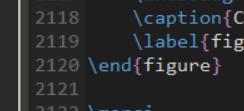
\includegraphics[width=0.8\textwidth]{figures/Rendu_5/Le_nouveau_rendu_/default/fig4.png}
    \caption{Caption here}
    \label{fig:Rendu_5_Le_nouveau_rendu__4}
\end{figure}

\begin{itemize}
	\item
	\item
\end{itemize}



\begin{figure}[h!]
    \centering
    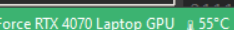
\includegraphics[width=0.8\textwidth]{figures/Rendu_5/Le_nouveau_rendu_/default/fig1.png}
    \caption{Caption here}
    \label{fig:Rendu_5_Le_nouveau_rendu__1}
\end{figure}


\begin{figure}[h!]
    \centering
    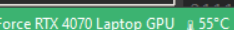
\includegraphics[width=0.8\textwidth]{figures/Rendu_5/Le_nouveau_rendu_/default/fig2.png}
    \caption{Caption here}
    \label{fig:Rendu_5_Le_nouveau_rendu__2}
\end{figure}


\begin{figure}[h!]
    \centering
    
\includegraphics[width=0.8\textwidth]{figures/Rendu_5/Le_nouveau_rendu_/default/fig3.png}
    \caption{Caption here}
    \label{fig:Rendu_5_Le_nouveau_rendu__3}
\end{figure}

\merci

\end{document}














































